\documentclass[crop, tikz]{standalone}

\usepackage[utf8]{inputenc}
% 'crop' is the default for v1.0, before it was 'preview'
%\usetikzlibrary{...}% tikz package already loaded by 'tikz' option

\usetikzlibrary{arrows}
\usetikzlibrary{decorations.markings}

\begin{document}
	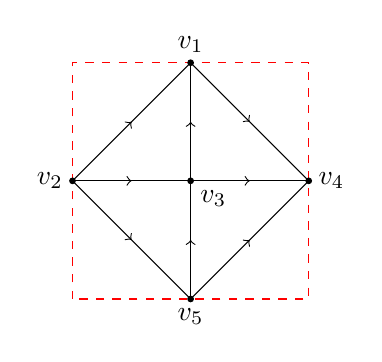
\begin{tikzpicture}[]
		\draw[dashed, red] (0,0) rectangle (3,3);
		\begin{scope}[decoration={markings, mark=at position 0.5 with {\arrow{>}}}]
			\draw[black, postaction={decorate}] (0,1.5) -- (1.5,1.5);
			\draw[black, postaction={decorate}] (1.5,1.5) -- (3,1.5);
			\draw[black, postaction={decorate}] (1.5,0) -- (1.5,1.5);
			\draw[black, postaction={decorate}] (1.5,1.5) -- (1.5,3);
			\draw[black, postaction={decorate}] (0, 1.5) -- (1.5,3);
			\draw[black, postaction={decorate}] (1.5,3) -- (3,1.5);
			\draw[black, postaction={decorate}] (0,1.5) -- (1.5,0);
			\draw[black, postaction={decorate}] (1.5,0) -- (3,1.5);
		\end{scope}
	
		%vertices, numbering is from TL -> TR - ML -> MR -> BL -> BR
		\filldraw[black] (1.5,3) circle (1pt) node[anchor=south] {$v_1$};
		\filldraw[black] (0,1.5) circle (1pt) node[anchor=east] {$v_2$};
		\filldraw[black] (1.5,1.5) circle (1pt) node[anchor=north west] {$v_3$};
		\filldraw[black] (3,1.5) circle (1pt) node[anchor=west] {$v_4$};
		\filldraw[black] (1.5,0) circle (1pt) node[anchor=north] {$v_5$};	
	\end{tikzpicture}
\end{document}